\begin{theo}[Elektromotorische “kracht”]{Elektromotorische “kracht”}
    Om stroom te hebben in een circuit, hebben we een apparaat nodig dat elektrische energie kan uitgeven. Dit apparaat wordt een bron van \textbf{elektromotorische kracht} (emf) genoemd.
    Het potentiaalverschil tussen de terminalen, ofwel de klemspanning, van de bron, wanneer er geen stroom vloeit, noemt men het emf $\mathcal{E}$ van de bron. Als er nu een stroom vloeit, dan is er een interne verzwakking van de klemspanning met een mate $Ir$ waarbij $r$ de interne weerstand is. In formulevorm krijgen we:
    \begin{equation*}
        \Delta V = \mathcal{E} - Ir
    \end{equation*}

    \begin{center}
        
        \begin{minipage}{.3 \textwidth}
            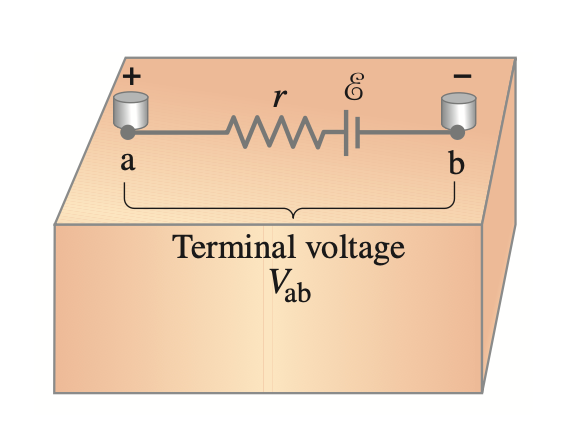
\includegraphics[scale = 0.45]{Images/Elektriciteit/Source.png}
        \end{minipage}
        \begin{minipage}{.3 \textwidth}
            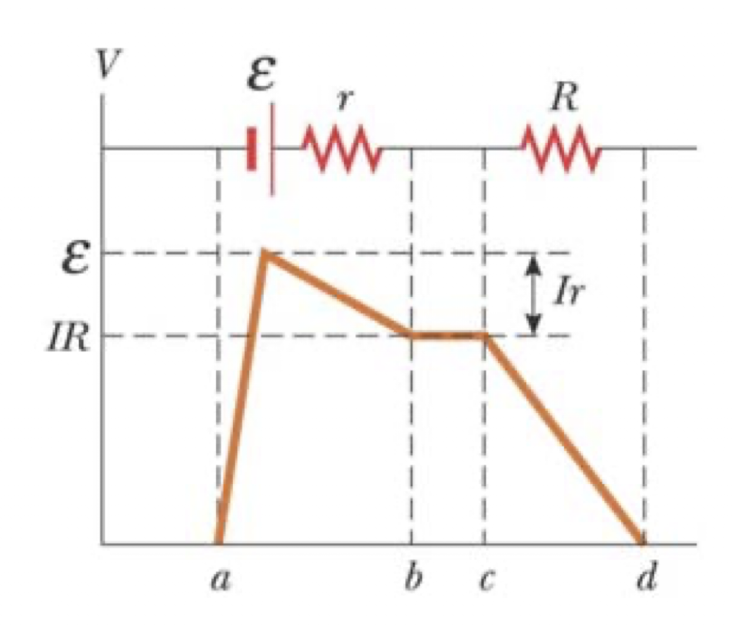
\includegraphics[scale = 0.35]{Images/Elektriciteit/EMFgrafiek.png}
        \end{minipage}

    \end{center}

    \vspace{-0.5cm}
    % \noindent \textbf{Opmerking:} de kracht in elektromotorische kracht staat niet voor een newtoniaanse kracht, het betekent eerder dat het een drijfveer is voor de elektrishe stroom.
\end{theo}

\begin{pro}[Weerstanden bij gelijkstroomschakelingen]{Weerstanden bij gelijkstroomschakelingen}
    \begin{center}
        \def\arraystretch{1.5}
        \begin{tabular}{c|c}
             Parallel & Serie \\ \hline
             $ I = \sum_i I_i $ & $ I = I_i$ \\
             $ \dfrac{1}{R} = \sum_i \dfrac{1}{R_i} $ & $R = \sum_i R_i$ \\
             $ \Delta V = \Delta V_i $ &  $ \Delta V = \sum_i \Delta V_i $
        \end{tabular}
    \end{center}
\end{pro}

% \begin{pro}[Weerstanden in serie bij gelijkstroomschakelingen]{Weerstanden in serie}
%     \begin{itemize}
%         \item $ I = I_i $
%         \item $ R = \sum_i R_i $
%         \item $ \Delta V = \sum_i \Delta V_i $
%     \end{itemize}
% \end{pro}

% \begin{pro}[Weerstanden in parallel bij gelijkstroomschakelingen]{Weerstanden in parallel}
%     \begin{itemize}
%         \item $ I = \sum_i I_i $
%         \item $ \dfrac{1}{R} = \sum_i \dfrac{1}{R_i} $
%         \item $ \Delta V = \Delta V_i $
%     \end{itemize}
% \end{pro}

\begin{theo}[Eerste regel van Kirchhoff]{Eerste regel van Kirchhoff}
     De som van de stromen die een vertakking binnenkomen, moet gelijk zijn aan de som van de stromen die de vertakking verlaten. In formulevorm:
     \begin{equation*}
         \sum I_{in} = \sum I_{uit}
     \end{equation*}
     \vspace{-0.5cm}
\end{theo}

\begin{theo}[Tweede regel van Kirchhoff]{Tweede regel van Kirchhoff}
    De som van de potentiaalverschillen over alle elementen in een gesloten kring, moet nul zijn. In formulevorm:
    \begin{equation*}
        \sum_{\text{gesloten kring}} \Delta V = 0
    \end{equation*}
    \vspace{-0.4cm}
\end{theo}

\newpage

\begin{app}[RC-kringen]{RC-kringen}
    Als de schakelaar dicht is, dan laadt de condensator op tot het het potentiaalverschil heeft van de batterij.
    We kunnen hierop de tweede regel van Kirchhoff toepassen, namelijk $\mathcal{E} - \dfrac{q}{C} - IR = 0$:
    \begin{align*}
        t &= 0: \mathcal{E} - I_0R = 0 \\ 
        t &= \infty: \mathcal{E} - \dfrac{Q}{C} = 0
    \end{align*}
    \begin{center}
        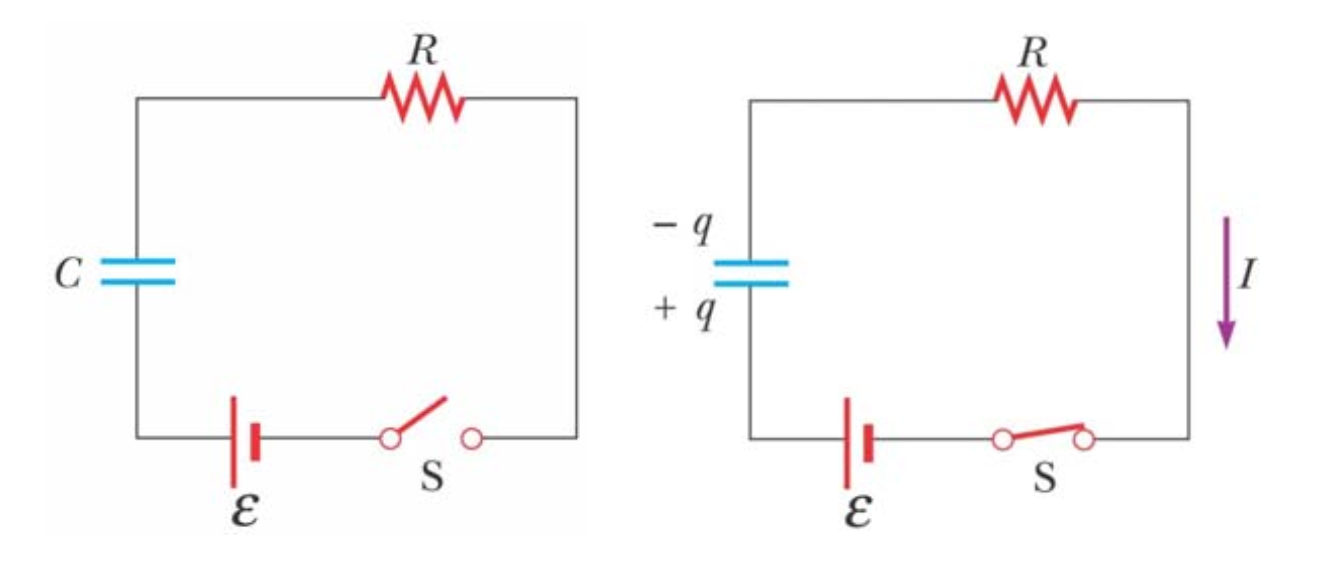
\includegraphics[scale = 0.3]{Images/Elektriciteit/RC-kring.png}
    \end{center}
    We weten dat stroom lading per tijdseenheid is dus we kunnen hieruit de volgende tijdsafhankelijke oplossingen halen:
    % \begin{align*}
    %     q &= C\mathcal{E}(1-e^{-\tfrac{t}{RC}})= Q(1-e^{-\tfrac{t}{RC}}) \\
    %     I &= \dfrac{dq}{dt} = \dfrac{\mathcal{E}}{R}e^{-\tfrac{t}{RC}}
    % \end{align*}

    \begin{equation*}
         I = \dfrac{dq}{dt} = \dfrac{d}{dt} C\mathcal{E}(1-e^{-\tfrac{t}{RC}}) = \dfrac{\mathcal{E}}{R}e^{-\tfrac{t}{RC}}
    \end{equation*}
    % \newpage
    
    \noindent We kunnen nu een nieuwe constante bepalen, namelijk de \textbf{tijdsconstante} $\tau = RC 
    % = \dfrac{\Delta V }{I}\dfrac{Q}{\Delta V}
    $    
    % \\
    % \begin{minipage}{0.48\textwidth}
    %     \centering
    %     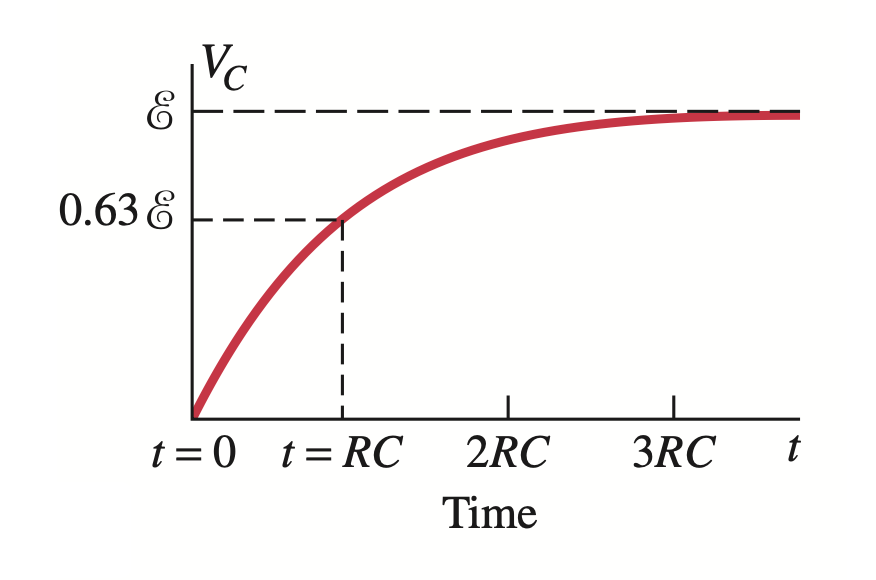
\includegraphics[scale = 0.2]{Images/Elektriciteit/Tijdsconstante1.png}
    % \end{minipage}
    % \begin{minipage}{0.48\textwidth}
    %     \centering
    %     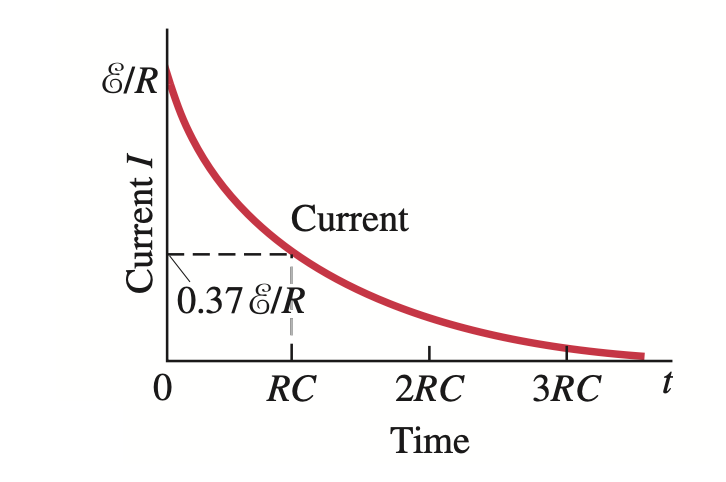
\includegraphics[scale = 0.23]{Images/Elektriciteit/Tijdsconstante2.png}
    % \end{minipage}
    % \\
    die de tijd voorstelt nodig voor een condensator om tot $ 63\%$ van zijn lading en voltage te bekomen: $RC$ is een maateenheid voor de snelheid van het opladen van de condensator. \\
    
    \noindent We kunnen ook wat praten over de energiebalans van de RC-kring: 
    \begin{itemize}
        \item Hoeveel energie heeft de emf geleverd? 
        \begin{equation*}
            U_{\text{emf}} = \int_0^Q \mathcal{E} dq = Q\mathcal{E} = \mathcal{E}^2C
        \end{equation*}
        \item Hoeveel energie is er opgeslagen in de condensator?
        \begin{equation*}
            U_{C} = \dfrac{\mathcal{E}^2C}{2} = \dfrac{Q^2}{2C}
        \end{equation*}
        \item Hoeveel warmte is er gedisipeerd in de weerstand?
        \begin{equation*}
            U_{R} = \dfrac{\mathcal{E}^2C}{2} = \dfrac{Q^2}{2C}
        \end{equation*}
    \end{itemize}
    We zien dus dat de energie geleverd door de emf netjes is verdeeld over de weerstand en de condensator, namelijk:
    \begin{equation*}
        U_{\text{emf}} = U_{C} + U_{R}
    \end{equation*}
\end{app}